\section{Protocolo v2 e validação automatizada}
\label{sec:v2}
\subsection{Resolução comum e rastreabilidade}
As limitações identificadas na avaliação histórica motivaram a implementação de um segundo protocolo. Em v2, cada caso usa a mesma largura e altura no alvo de temporização, na captura RGBA, no cálculo de PSNR/SSIM e na telemetria. O par de imagens para ambas as métricas é o mesmo; a máscara de terreno vem do canal alfa. A etapa Python confere as dimensões reais dos PNGs, recalcula PSNR e verifica sua concordância com o valor obtido no navegador, com tolerâncias absoluta e relativa de $10^{-9}$. O SSIM usa a janela $11\times11$ e exclui centros cujo suporte ultrapasse o terreno ou a imagem, sem recorrer a uma máscara menos restritiva quando não existem janelas válidas.

A leitura de pixels e a codificação das imagens ocorrem antes da temporização. O passe temporizado continua incluindo terreno e céu, enquanto as métricas consideram apenas o terreno. Cada captura é exportada por etapas para evitar acumular múltiplas imagens 4K simultaneamente em memória. Os arquivos registram dimensões, método, referência, estimador de seleção e filtro inicial, e os validadores rejeitam resultados com resoluções incompatíveis ou células ausentes na matriz de métodos.

O registro de consultas foi substituído por um histórico individual com identificadores de sessão, caso, método, rodada e posição na ordem de execução. Cada consulta preserva fase, instante de submissão, disponibilidade, estado de disjunção e, quando válida, duração em nanossegundos e milissegundos. Os estados finais distinguem coleta válida, aquecimento válido, disjunção, expiração e resultado inválido. Uma disjunção invalida todas as consultas pendentes, inclusive aquelas ainda indisponíveis, evitando que uma consulta contaminada seja aceita em uma leitura posterior.

Para cada método, a contagem de consultas solicitadas deve ser igual à soma de válidas e descartadas. Os agregados são recalculados a partir das consultas aceitas; aquecimento não entra nas estatísticas. São exportados média, mediana, quartis, IQR, P95, desvio padrão descritivo e causas de descarte. O protocolo científico exige o timer de GPU, sem substituição silenciosa por um cronômetro de CPU. O runner identifica renderização por software, que é tolerada apenas quando explicitamente habilitada para validação funcional.

O comando de coleta completa foi configurado para cinco sessões, cada uma em um processo e perfil novos de navegador. Por caso, o padrão é de 60 renderizações iniciais, cinco rodadas de aquecimento e 100 rodadas de coleta, com ordem direta/reversa alternada. O resumo mantém as medianas de cada sessão e calcula sua mediana e IQR entre sessões, sem tratar consultas de uma mesma sessão como repetições independentes. Esses valores são escolhas explícitas de protocolo; sua implementação não demonstra, por si só, convergência do aquecimento ou estabilidade estatística.

\subsection{Ablação e controle negativo}
A Equação~\ref{eq:lodseparado} permite uma matriz fatorial $2\times2$: estimador de seleção isotrópico ou anisotrópico, combinado com filtragem inicial por \texttt{textureGrad} ou \texttt{textureLod}. O LOD usado na amostragem dos níveis posteriores permanece anisotrópico e fixo entre as células. Os identificadores \texttt{adap\_iso} e \texttt{adap\_aniso} agora compartilham o filtro inicial \texttt{grad}; as duas células adicionais usam o sufixo \texttt{\_lod}. Por isso, os números antigos de \texttt{adap\_iso} não são intercambiáveis com os de v2, apesar da semelhança do nome.

Além de conferir parâmetros, implementamos um controle negativo sobre imagens realmente renderizadas. Nele, os limiares são elevados para $n=2$ e $f=3$, acima de $\xi\in[0,\,1]$, mantendo todos os fragmentos no regime completo. Com pesos de regime constantes, trocar somente o estimador de seleção deve produzir os mesmos pixels para um filtro fixo. O teste exige identidade contra a referência nas células \texttt{grad}, com PSNR infinito e SSIM unitário, e igualdade dos PNGs entre as duas células \texttt{lod}. O controle passou nos dois enquadramentos de teste. Ele detectaria o acoplamento anterior em que o estimador alterava também os mipmaps amostrados, embora não substitua a análise de todas as condições possíveis.

\subsection{Suíte e resultados funcionais}
A suíte de validação combina casos em Node.js (\texttt{node:test}) e em Python, executados sob \texttt{npm test}. Foram aprovados 25 testes automatizados, um dos quais executa cinco verificações em Python com valores de referência de PSNR/SSIM, máscara e suporte da janela. Os demais verificam a matriz de ablação, as estatísticas, a exclusão de aquecimento, a preservação de consultas, os estados de descarte e a rejeição de relatórios inconsistentes. Testes com contexto de GPU simulado exercitam disjunção antes da disponibilidade e expiração; os testes de integração usam o shader real.

As integrações foram executadas em Chrome headless 136, Windows, WebGL 2 via ANGLE/D3D11, sobre uma NVIDIA GeForce RTX 4050 Laptop GPU, com suporte ao timer de GPU. O ambiente de orquestração usou Node.js 24.11.1 e Python 3.12.14. Os dois testes de \texttt{npm run test:gpu} cobrem duas sessões independentes em $320\times180$ e $640\times360$, seguidas do controle negativo em uma terceira sessão. O teste \texttt{npm run test:gpu:resolutions} acrescenta uma quarta sessão, com panorâmica em 1080p e rasante em 4K. Todas as quatro sessões foram concluídas.

Foram preservados 288 registros de consultas: 216 de coleta válidas e 72 de aquecimento válido, sem descartes nesses casos. Cada sessão cobre 18 combinações de caso/método, incluindo as quatro células adaptativas e cinco comparadores. A configuração curta usa três rodadas de coleta e uma de aquecimento por método, além de seis renderizações iniciais. Ela verifica execução e consistência; não constitui a coleta científica de cinco sessões e 100 rodadas descrita anteriormente.

\begin{table*}[t]
\centering\small\setlength{\tabcolsep}{4pt}
\caption{Validação funcional do protocolo v2 na RTX 4050. PSNR e SSIM usam as mesmas capturas RGBA e dimensões da temporização. Os enquadramentos diferem entre as colunas; esta tabela não mede escalabilidade de resolução. Cada linha tem três consultas de coleta válidas por caso, sem descartes.}
\label{tab:v2quality}
\begin{tabular}{lrrrr}\toprule
 & \multicolumn{2}{c}{1080p, panorâmica} & \multicolumn{2}{c}{4K, rasante}\\
Método & PSNR (dB) & SSIM & PSNR (dB) & SSIM\\\midrule
Linear & 32,65 & 0,963659 & 31,17 & 0,985847\\
Completo 6 & $\infty$ & 1,000000 & $\infty$ & 1,000000\\
Truncado 3 & 32,52 & 0,957478 & 31,76 & 0,985509\\
Salto par & 51,99 & 0,999317 & 50,03 & 0,999633\\
Híbrido & 37,09 & 0,984116 & 36,89 & 0,994978\\
Adaptativo iso./grad & 35,12 & 0,969095 & 40,03 & 0,990984\\
Adaptativo aniso./grad & 42,18 & 0,988397 & 50,77 & 0,998220\\
Adaptativo iso./lod & 28,02 & 0,844573 & 29,52 & 0,927398\\
Adaptativo aniso./lod & 28,90 & 0,858891 & 29,96 & 0,931633\\
\bottomrule\end{tabular}
\end{table*}


A Tabela~\ref{tab:v2quality} apresenta as métricas das capturas coincidentes com as resoluções temporizadas. Com filtro inicial \texttt{grad} mantido constante, o adaptativo anisotrópico obtém 42,18 dB contra 35,12 dB do isotrópico na panorâmica a 1080p, e 50,77 contra 40,03 dB na rasante a 4K. Os SSIMs correspondentes são, respectivamente, 0,988397 contra 0,969095 e 0,998220 contra 0,990984. Esses dois casos fornecem evidência de uma diferença de fidelidade associada à seleção de regimes sob filtragem controlada. Não estabelecem superioridade em materiais ou enquadramentos não avaliados.

As células \texttt{lod} apresentam PSNR menor contra a referência comum \texttt{grad}, evidenciando que a filtragem inicial é um fator distinto e relevante. A comparação não atribui todo esse desvio à política adaptativa, pois a própria referência usa outro filtro. O salto par permanece próximo da referência, com 51,99 dB na panorâmica a 1080p e 50,03 dB na rasante a 4K. A Figura~\ref{fig:v2frames} mostra as capturas com filtragem inicial constante.

\begin{figure*}[t]
\centering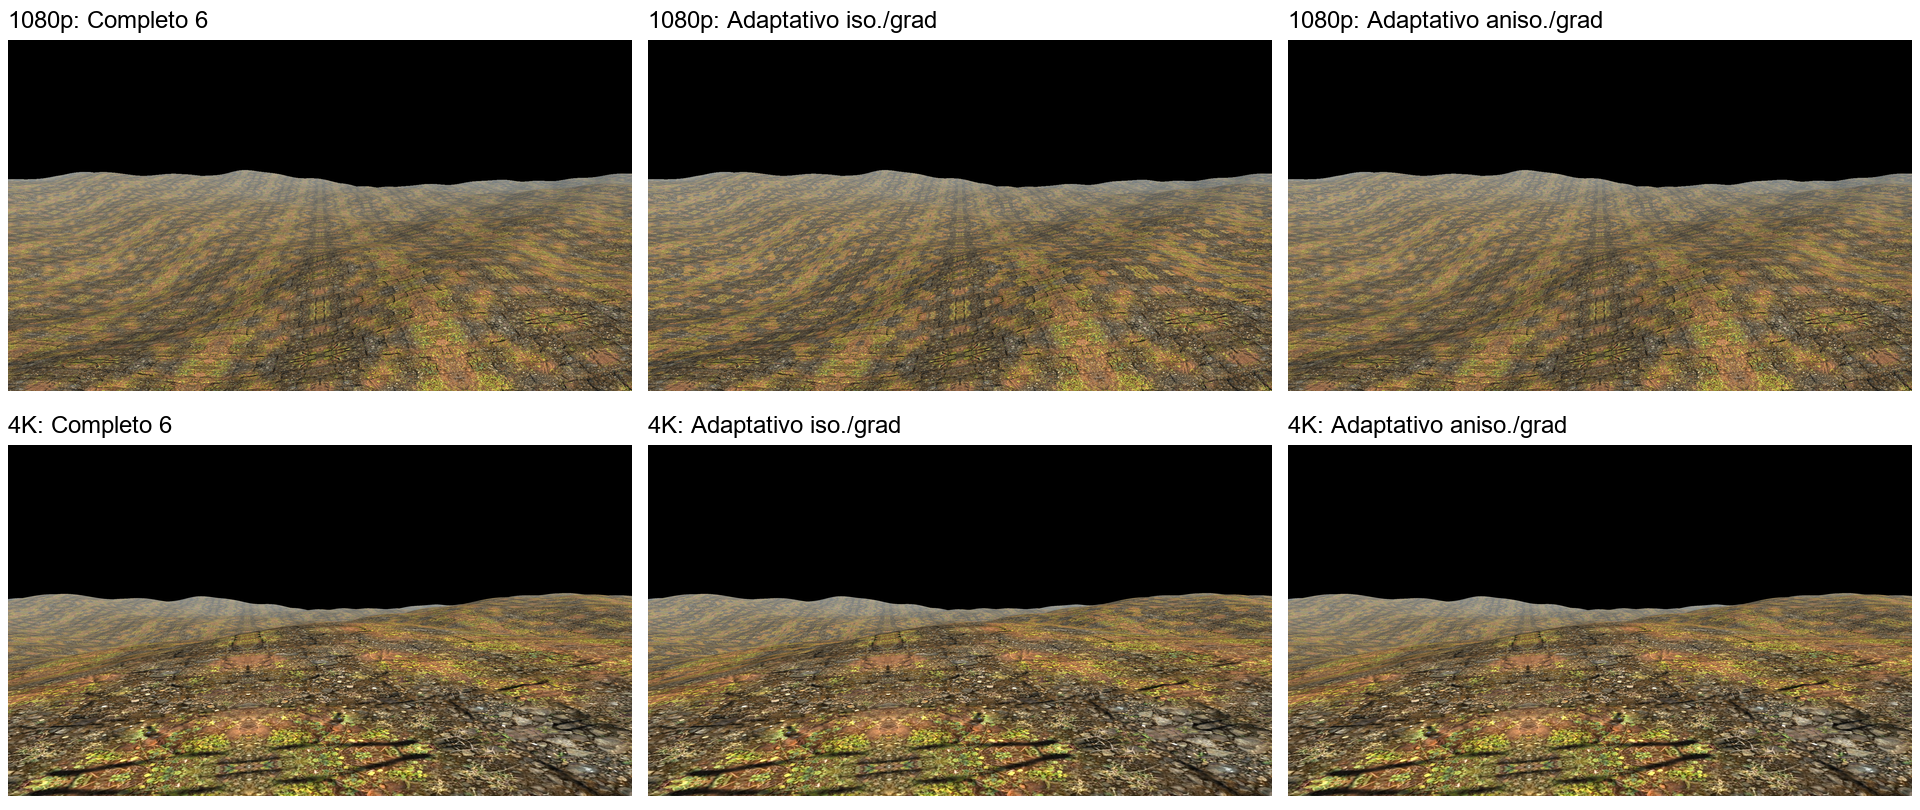
\includegraphics[width=0.97\textwidth]{figures/validacao_v2.png}
\caption{Capturas do protocolo v2 na RTX 4050: completo, adaptativo isotrópico e adaptativo anisotrópico, todos com filtro inicial \texttt{grad}. Linha superior: panorâmica a 1080p; inferior: rasante a 4K. As imagens foram reduzidas apenas para compor a figura; as métricas usam os PNGs originais. O fundo preto corresponde aos pixels fora do terreno excluídos pela máscara alfa.}
\label{fig:v2frames}
\end{figure*}

Os tempos individuais da coleta curta são disponibilizados para auditoria da instrumentação, mas não usados para anunciar novas reduções de desempenho ou comparar a RTX 4050 com a GPU AMD histórica. Além da troca de hardware, o algoritmo de seleção/filtragem e o protocolo mudaram. O ganho principal demonstrado nesta etapa é metodológico: as dimensões coincidem, as consultas podem ser auditadas e o fator de seleção possui um controle de independência em pixels. A coleta completa permanece necessária para concluir sobre estabilidade dos tempos e o novo compromisso custo--qualidade.
